\newpage\subsection*{1551 Worksheet 4 Answers}

\SolutionsStatement

\begin{enumerate}
    
    \item \begin{enumerate} 
    	\item False. The graph of a function can cross a horizontal asymptote. For example: $1+\sin(t)/t$. 
    	\item True. The limit of the product is the product of the limits:
        \begin{align*}
        	\lim_{t\rightarrow 2} \ t^2 \, f(t) &= \infty\\
            \lim_{t\rightarrow 2} \ t^2 \, \lim_{t\rightarrow 2} f(t) &= \infty\\
            4 \, \lim_{t\rightarrow 2} f(t) &= \infty\\
            \lim_{t\rightarrow 2} f(t) &= \infty
        \end{align*}
        \item False. Because $\sqrt{a+b} \ne \sqrt{a} + \sqrt{b}$ for all $a$ and $b$.
        \item False. Because $\infty - \infty$ is undefined. 
    \end{enumerate}
    The limit in parts (c) and (d) is explored in our textbook, \Textbook. See Example 9, Section 2.6, page 108. 
    
    \item \begin{enumerate}
    	\item Possible, see graph below. 
		\begin{center}
			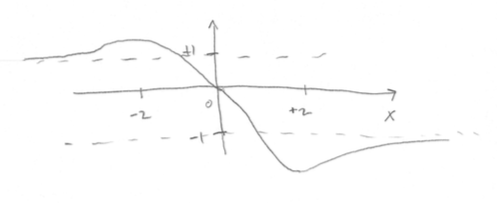
\includegraphics[width=0.8\textwidth]{images/imgWS4Spring17.png} 
		\end{center}
    
        \item Impossible. If $g$ is even, then $g$ is symmetric about the line $x=0$, so 
        $$\lim_{x\rightarrow\infty} g(x) = \lim_{x\rightarrow-\infty} g(x)$$
    \end{enumerate}    
    
    \item \begin{enumerate}\setlength\itemsep{12pt}
    
		\item $\displaystyle{\lim_{x\to 5^-} \left(\frac{3x}{2x-10}\right)} = -\infty$

		\item $\displaystyle{\lim_{t\to \infty}\ln\left(1+\frac{1}{t}\right)}
 = \ln(1 + 0) = \ln(1) = 0 $
 
		\item \begin{align*} 
        	\lim_{x\to \infty} \left(\frac{2+\sqrt{x}}{2-\sqrt{x}}\right) &= 
        	\lim_{x\to \infty} \left(\frac{2+\sqrt{x}}{2-\sqrt{x}}\right)\left(\frac{2-\sqrt{x}}{2-\sqrt{x}}\right) \\ &=
            \lim_{x\to \infty} \left(\frac{4-x}{4-2\sqrt{x}+x}\right)  \\ &= 
            \lim_{x\to \infty} \left(\frac{4/x-1}{4/x-\frac{2}{\sqrt{x}}+1}\right)  \\ &= 
            \frac{-1}{1} \\ &= 
            -1
            \end{align*}

	\end{enumerate}

	\item Horizontal asymptotes: 
    \begin{align*} 
    	\lim_{x\to \pm \infty } \left(\frac{x^3-4x^2+3x}{3x^2-6x}\right) = \pm \infty 
    \end{align*}
    Therefore no horizontal asymptotes. Vertical asymptotes: 
	\begin{align*} 
    	\frac{x^3-4x^2+3x}{3x^2-6x} &= \frac{x^2-4x+3}{3x-6}\\
        &= \frac{(x-1)(x-3)}{3x-6}\\
    	\lim_{x\to 2 ^- } \frac{(x-1)(x-3)}{3x-6} &= +\infty \\
    	\lim_{x\to 2 ^+ } \frac{(x-1)(x-3)}{3x-6} &= -\infty 
    \end{align*}
	For the oblique asymptotes, use polynomial division to obtain:
    \begin{align*} 
    	f(x) &= \frac{x^2-4x+3}{3x-6} = \frac x 3 - \frac 2 3 - \frac{1}{3x - 6}
    \end{align*}
	Thus, $f$ has the oblique asymptote $\frac x 3 - \frac 2 3$.
    
    \item 
    \begin{enumerate}
    	\item \begin{align*}
        \text{average speed at time } t \text{ over interval } [t,t+\Delta t]&= \frac{(t+\Delta t)^2 + 2(t+\Delta t) - (t^2 + 2t)}{\Delta t} \\
        &= \frac{ (\Delta t)^2 + 2 \Delta t\, t + 2 \Delta t}{\Delta t} \\
        &= \Delta t + 2t + 2 \\
		\text{average speed at time } 1 \text{over interval } [1,1+\Delta t]
        &= \Delta t + 2(1) + 2 \\ 
        &= \Delta t + 4
        \end{align*}
        \item $\Delta t = 1$, so average speed over $[1,2]$ is $\Delta t+4 = 5$. 
        \item instantaneous speed at $t = 1$ is $$\lim_{\Delta t \rightarrow 0} (\Delta t + 2t + 2 )\huge|_{t = 1} =  (0+2t + 2) \huge|_{t = 1} = 4$$
    \end{enumerate}
\end{enumerate}




